\chapter{Wyniki oraz omówienie}
\label{chap:wyniki}

W celu porównania obu rozwiązań przedstawionych w \autoref{chap:implementacja} przeprowadzono szereg testów.
Oceniono poprawność działania algorytmu na uproszczonych, automatycznie generowanych danych a także na podstawie
rzeczywistych danych pochodzących ze skanowania laserowego. Sprawdzono również czasy przetwarzania dla poszczególnych
algorytmów oraz stwierdzono, czy możliwe jest wykorzystanie obu algorytmów jednocześnie w celu poprawienia jakości wyników.

Wszystkie testy zostały przeprowadzone na komputerze, którego specyfikacje podano w tabeli \ref{tab:specyfikacja}.

\begin{table}[h!]
    \centering
    \begin{tabular}{|p{0.5\linewidth}|p{0.5\linewidth}|}
        \hline
        Procesor & Intel Core i5-6300U 2,4 GHz \\
        \hline
		Pamieć & 16GB \\
		\hline
		Dysk & Intel SSDSC2BB80 800GB \\
		\hline
		System Operacyjny & Fedora 23 kernel 4.6.3 \\
		\hline
		Interpreter Pythona & Python 2.7.11 \\
		\hline
    \end{tabular}
    \caption{Specyfikacja platformy testowej}
    \label{tab:specyfikacja}
\end{table}

\section{Testy na danych wygenerowanych}
Pierwszy z testów miał wykazać poprawność działania zaimplementowanych algorytmów. W tym celu wygenerowano zbiór 1000 punktów,
których współrzędne $x,y \in <0,1>$, zaś wartość wspólrzędnej $z$ dana jest wzorem:

\begin{displaymath}
    z = \left\{ \begin{array}{ll}
        r & \textrm{$x < 0,4 \vee x > 0,6 \vee y < 0,4 \vee y > 0,6$}\\
        1 + r & \textrm{$0,4 < x < 0,6 \wedge 0,4 < y < 0,6$}\\
    \end{array} \right.
\end{displaymath}


Gdzie $r$ jest zmienna losową z przedziału $<0;0,1>$. Tak utworzone dane powinny zostać zintepretowane jako
dwie niezależne płaszczyzny. Widok przykładowych danych w 3 wymiarach pokazano na rysunku \ref{fig:dane_zerowe}.

\begin{figure}[h!]
    \centering
    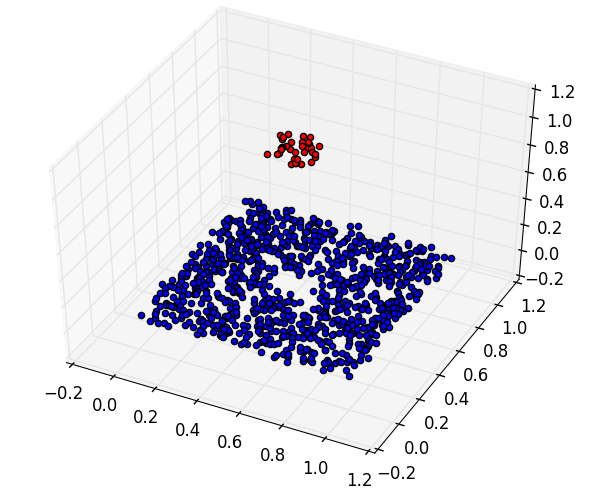
\includegraphics[width=0.6\linewidth]{img/test0.png}
    \caption{Dane testowe w rzucie 3D}
    \label{fig:dane_zerowe}
\end{figure}

Dane testowe oraz wyniki działania algorytmu przedstawiono na rysunkach \ref{fig:test1} i \ref{fig:test2}.
Przez kolor czerwony zostały oznaczone punkty dla których $z > 1$.

\begin{figure}[h!]
    \centering
    \begin{subfigure}[b]{0.5\linewidth}
        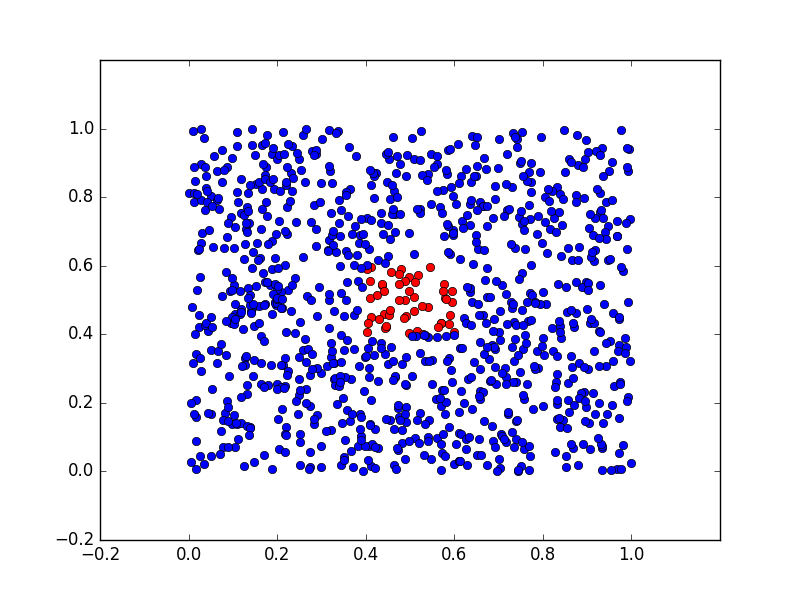
\includegraphics[width=\linewidth]{img/test1_1.png}
		\caption{Dane wejściowe}
    \end{subfigure}%
    \begin{subfigure}[b]{0.5\linewidth}
        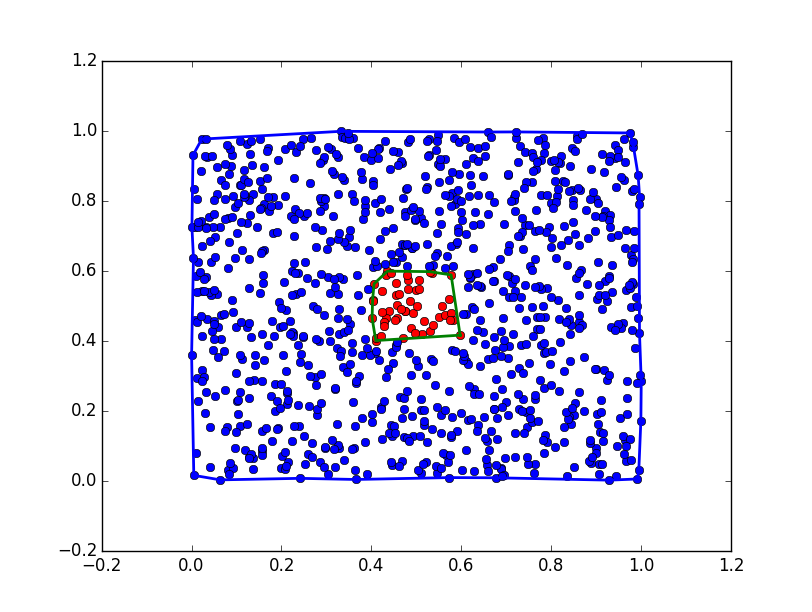
\includegraphics[width=\linewidth]{img/test1_2.png}
		\caption{Algorytm naiwny}
    \end{subfigure}%

    \begin{subfigure}[b]{0.5\linewidth}
        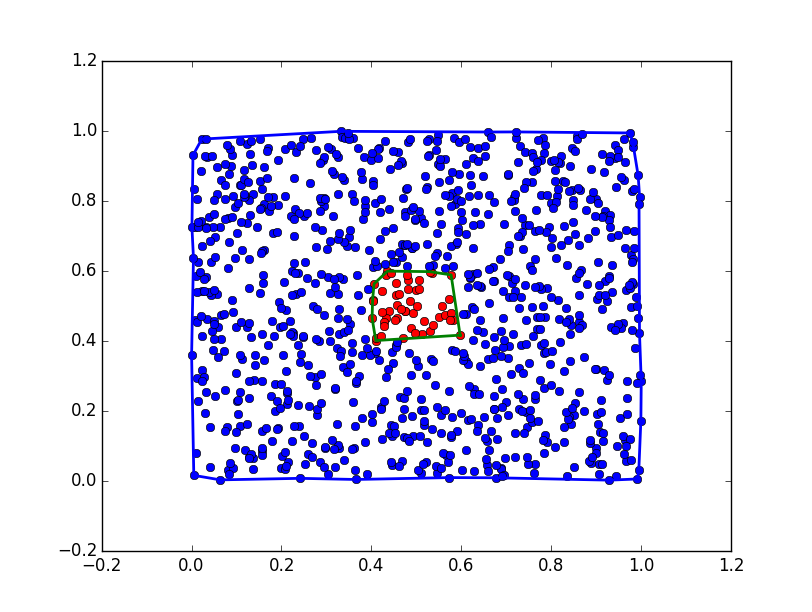
\includegraphics[width=\linewidth]{img/test1_3.png}
        \caption{Algorytm iteracyjny (1 iteracja)}
    \end{subfigure}%
    \caption{Wyniki działa algorytmu dla wygenerowanych danych testowych}
    \label{fig:test1}
\end{figure}

Jak widać na rysunku \ref{fig:test1} oba algorytmy poprawnie wykryły dwie powierzchnie. Co ciekawe,
algorytm iteracyjny już po pierwszej iteracji poprawnie zakwalifikował punkty do dwóch zbiorów. Niestety, jest to
dziełem przypadku, co zostało wykazane przez kolejny test.

\begin{figure}[h!]
    \centering
    \begin{subfigure}[b]{0.5\linewidth}
        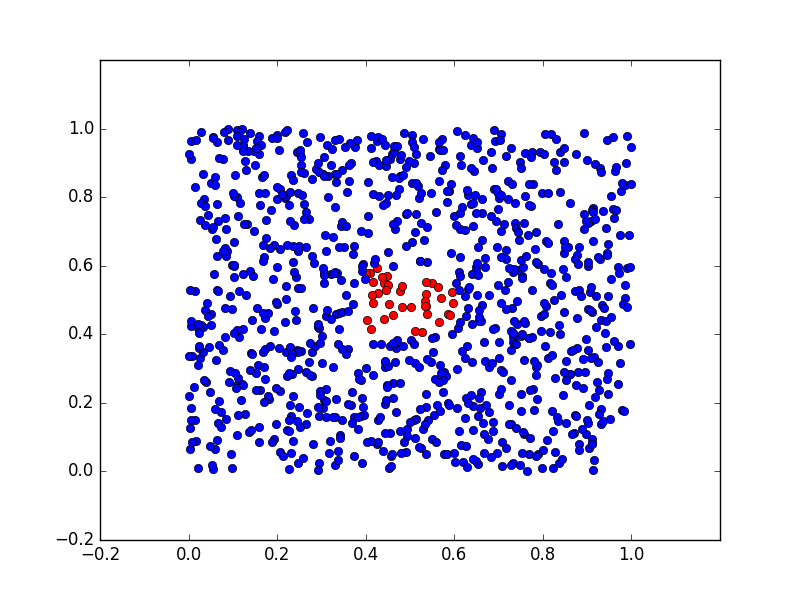
\includegraphics[width=\linewidth]{img/test2_1.png}
        \caption{Dane wejściowe}
    \end{subfigure}%
    \begin{subfigure}[b]{0.5\linewidth}
        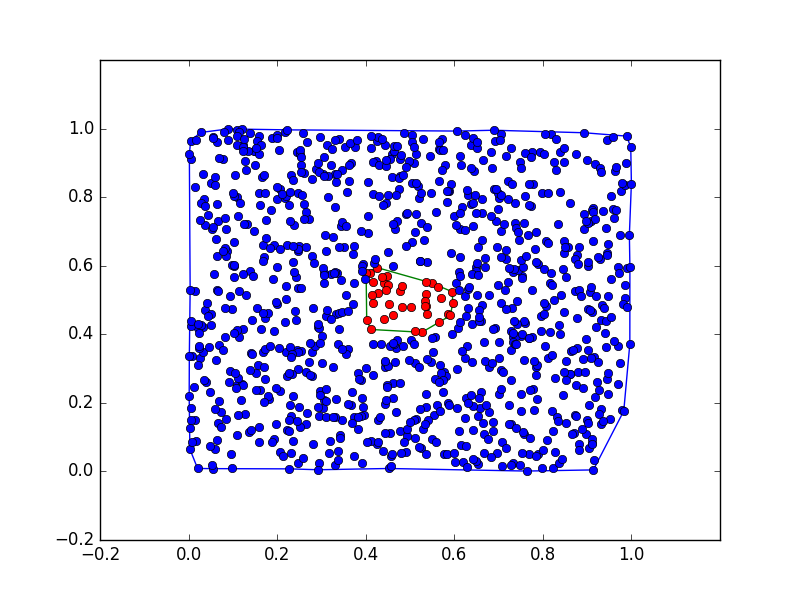
\includegraphics[width=\linewidth]{img/test2_2.png}
        \caption{Algorytm naiwny}
    \end{subfigure}%

    \begin{subfigure}[b]{0.5\linewidth}
        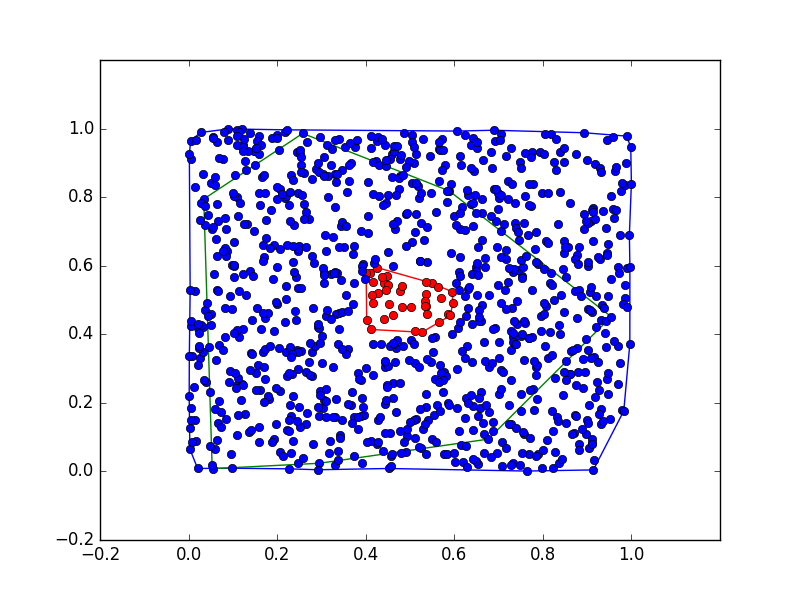
\includegraphics[width=\linewidth]{img/test2_3.png}
        \caption{Algorytm iteracyjny (1 iteracja)}
    \end{subfigure}%
    \begin{subfigure}[b]{0.5\linewidth}
        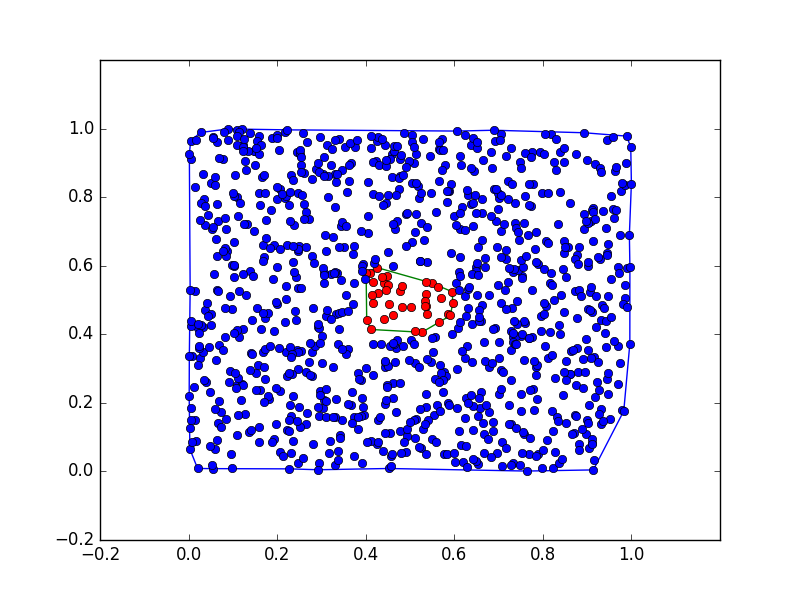
\includegraphics[width=\linewidth]{img/test2_4.png}
        \caption{Algorytm iteracyjny (7 iteracja)}
    \end{subfigure}%
    \caption{Wyniki działa algorytmu dla wygenerowanych danych testowych}
    \label{fig:test2}
\end{figure}

W przypadku pokazanym na rysunku \ref{fig:test2} koniecznych było 7 iteracji, aby w prawidłowy sposób wykryć, iż
w danych testowych znajdują się dwie powierzchnię. Przypadek ten pokazuje, że algorytm iteracyjny ma właściwości
poprawiania wyników wraz z kolejnymi iteracjami. Porównano także czasy wykonywania się algorytmów (tabela \ref{tab:czasy1})

\begin{table}[h!]
    \centering
    \begin{tabular}{|p{0.5\linewidth}|p{0.5\linewidth}|}
        \hline
        Algorytm Naiwny & 1,40s \\
        \hline
        Algorytm Iteracyjny - 1 iteracja & 15,47s \\
        \hline
        Algorytm Iteracyjny - 7 iteracji & 4min 33,08s (273,08s) \\
        \hline
        Algorytm Iteracyjny - 7 iteracji (średni czas 1 iteracji) & 39,01s \\
        \hline
    \end{tabular}
    \caption{Średnie czasy wykonywania sie algorytmu}
    \label{tab:czasy1}
\end{table}

Podsumowując - oba algorytmy dają poprawne wyniki. Algorytm naiwny jest ponad 10 razy szybszy w optymistycznym,
i nawet 195 razy szybszy w pesymistycznym przypadku niż algorytm iteracyjny. Z drugiej jednak strony, algorytm
naiwny nie ma możliwości poprawy wyników wraz z kolejnymi iteracjami, co może mieć krytyczne znaczenie przy
analizowaniu danych rzeczywistych.

\section{Testy na danych rzeczywistych}

Po sprawdzeniu poprawności działania obu algorytmów przystopiono do testów na prawdziwych danych.
Dane te zostały zebrane dnia 28 sierpnia 2012 roku w ramach programu ISOK. Obejmują swoim zasięgiem okolice
gmachu Elektroniki gmachu Oceanotechniki i Okrętownictwa oraz gmachu Mechaniki Politechniki Gdańskiej.
Dokładny zasięg danych został przedstawiony na rysunku \ref{fig:dane_testowe}.

\begin{figure}[h!]
    \centering
    \begin{subfigure}[b]{0.5\linewidth}
		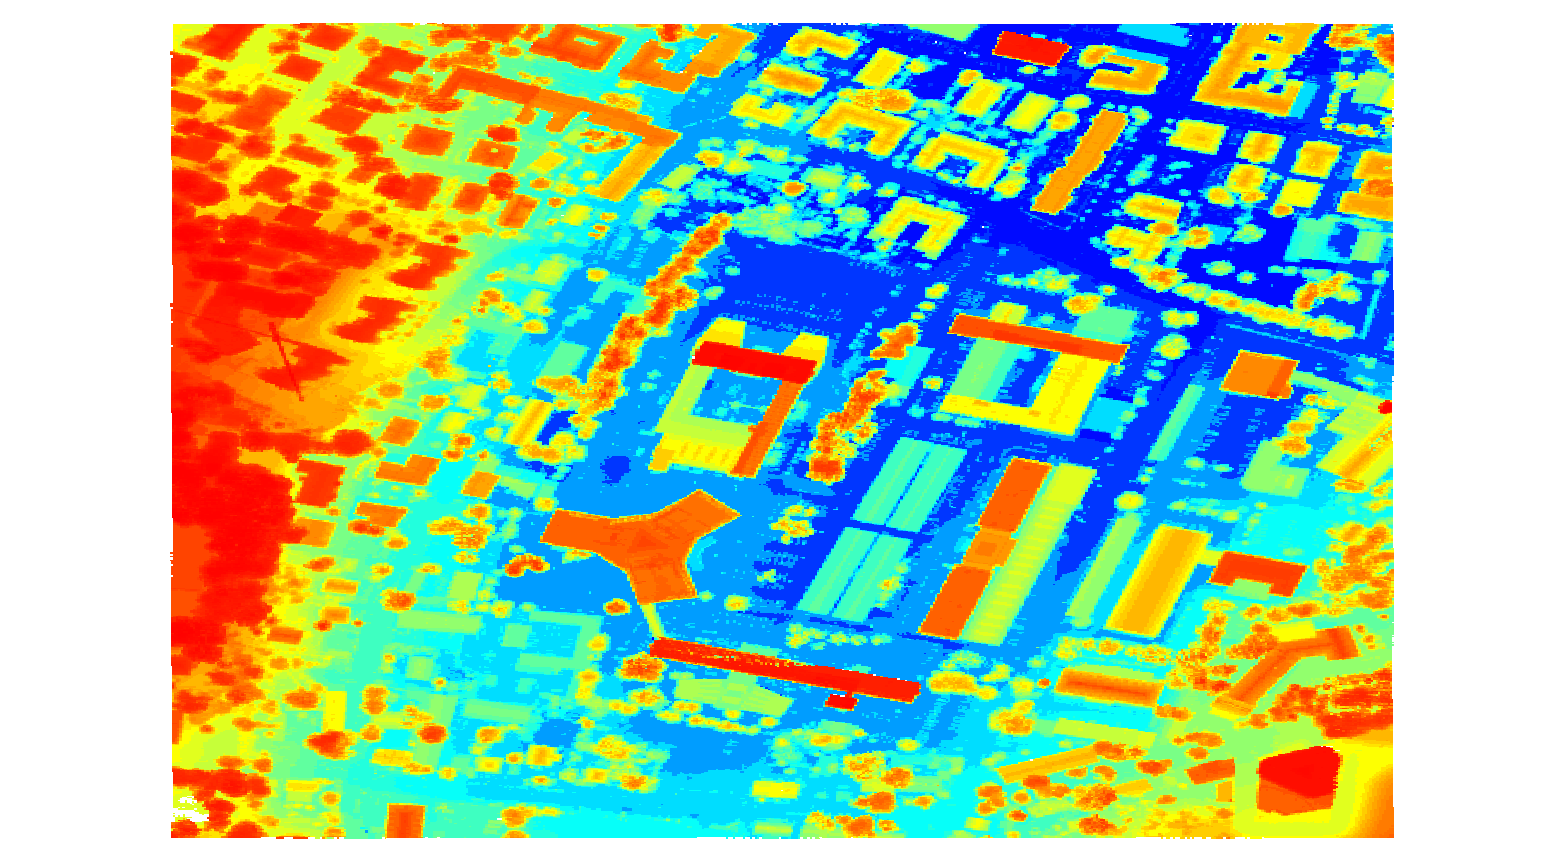
\includegraphics[width=\linewidth]{img/dane_testowe1.png}
        \caption{Dane testowe}
    \end{subfigure}%
    \begin{subfigure}[b]{0.5\linewidth}
        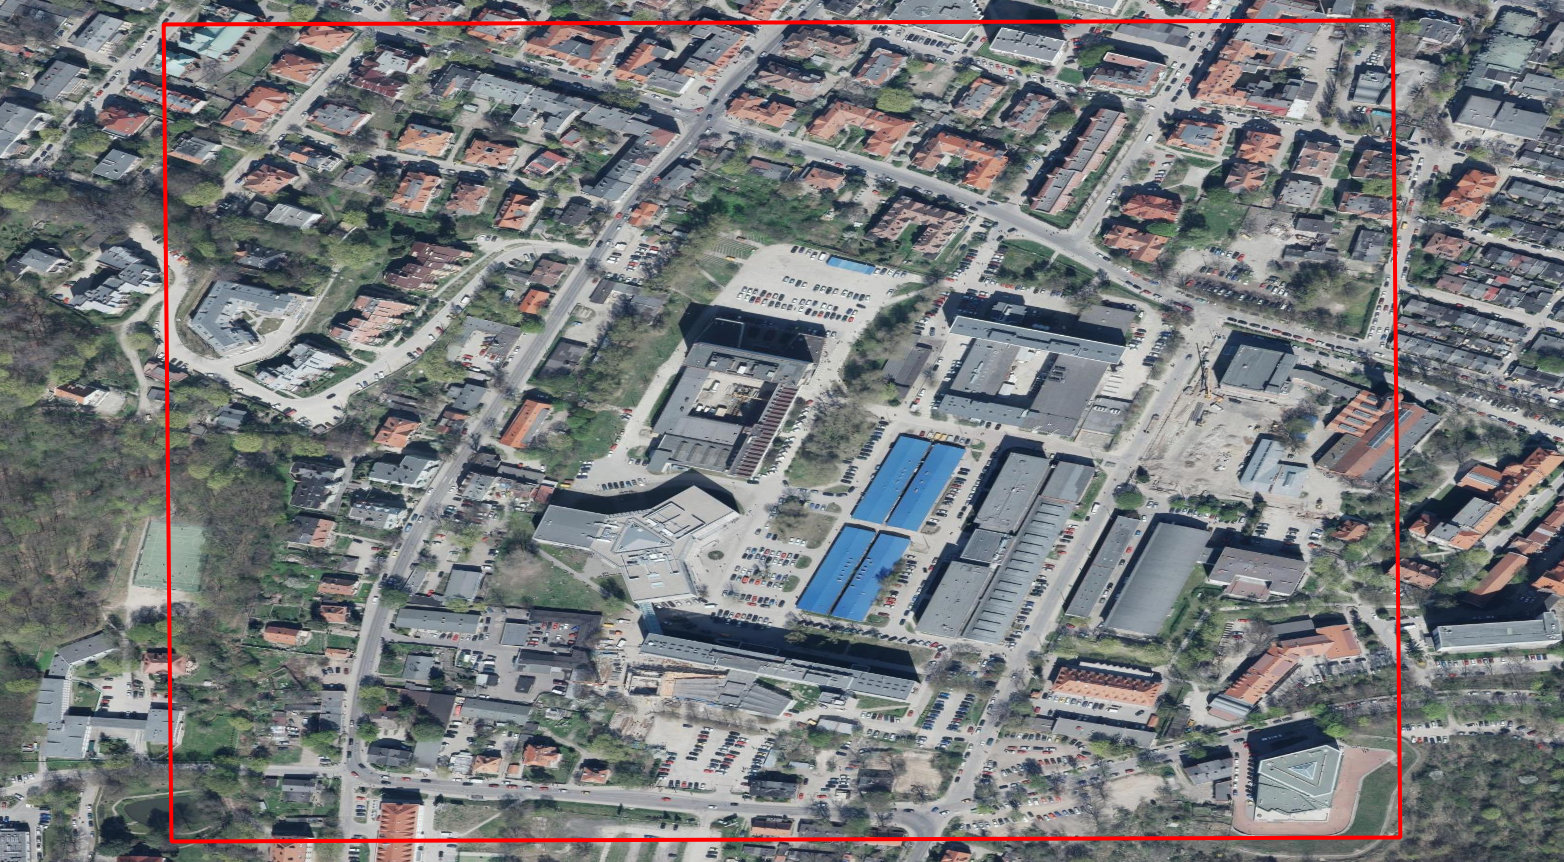
\includegraphics[width=\linewidth]{img/dane_testowe2.png}
        \caption{Obszar danych testowych zaznaczony na zdjęciu}
    \end{subfigure}%
    \caption{Obszar objęty przez dane testowy}
    \source{http://mapy.geoportal.gov.pl/wss/service/img/guest/ORTO/MapServer/WMSServer}
    \label{fig:dane_testowe}
\end{figure}

Dane zaprezentowane na rysunku \ref{fig:dane_testowe} wykorzystano jako dane wejściowe
dla przygotowanych algorytmów. Najpierw sprawdzono efekt działania algorytmu naiwnego.

\begin{figure}[h!]
    \centering
    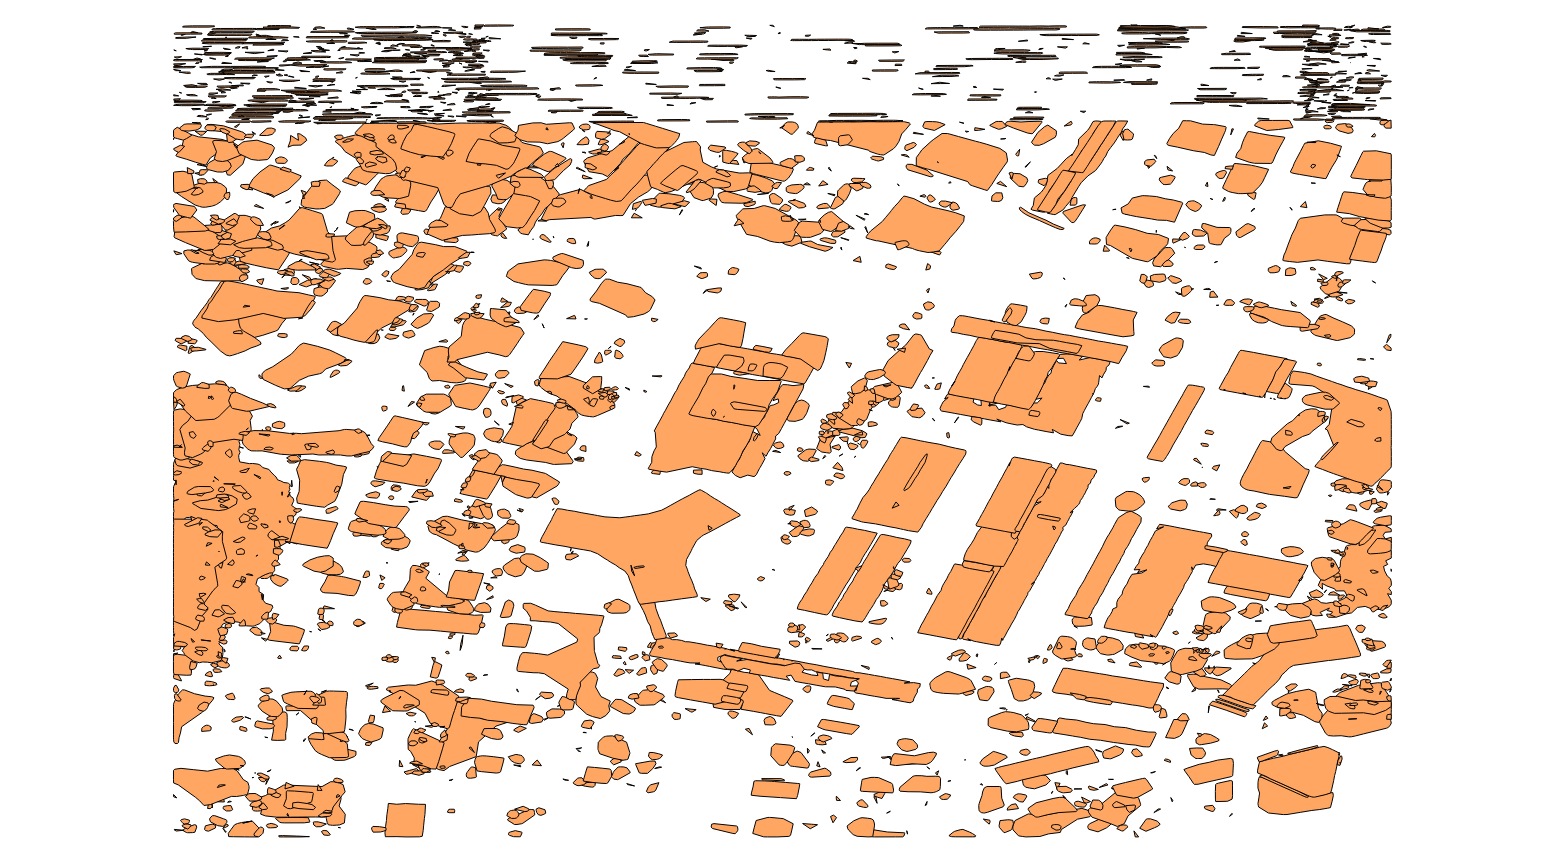
\includegraphics[width=\linewidth]{img/wynik_naiwny.png}
    \caption{Efekt działania algorytmu naiwnego}
    \label{fig:wynik_naiwny}
\end{figure}

Na rysunku \ref{fig:wynik_naiwny} przedstawiono efekty działania algorytmu naiwnego.
Na pierwszy rzut oka wydają się być poprawne. Widać wyraźnie zarysowany kształt budynku
nowej elektroniki. Niestety istnieje też wiele źle zidentyfikowanych fragmentów. Przede
wszystkim są to drzewa, a także nie wyjaśnione zakłócenia widoczne u góry rysunku.

\begin{figure}[h!]
    \centering
    \begin{subfigure}[b]{0.5\linewidth}
        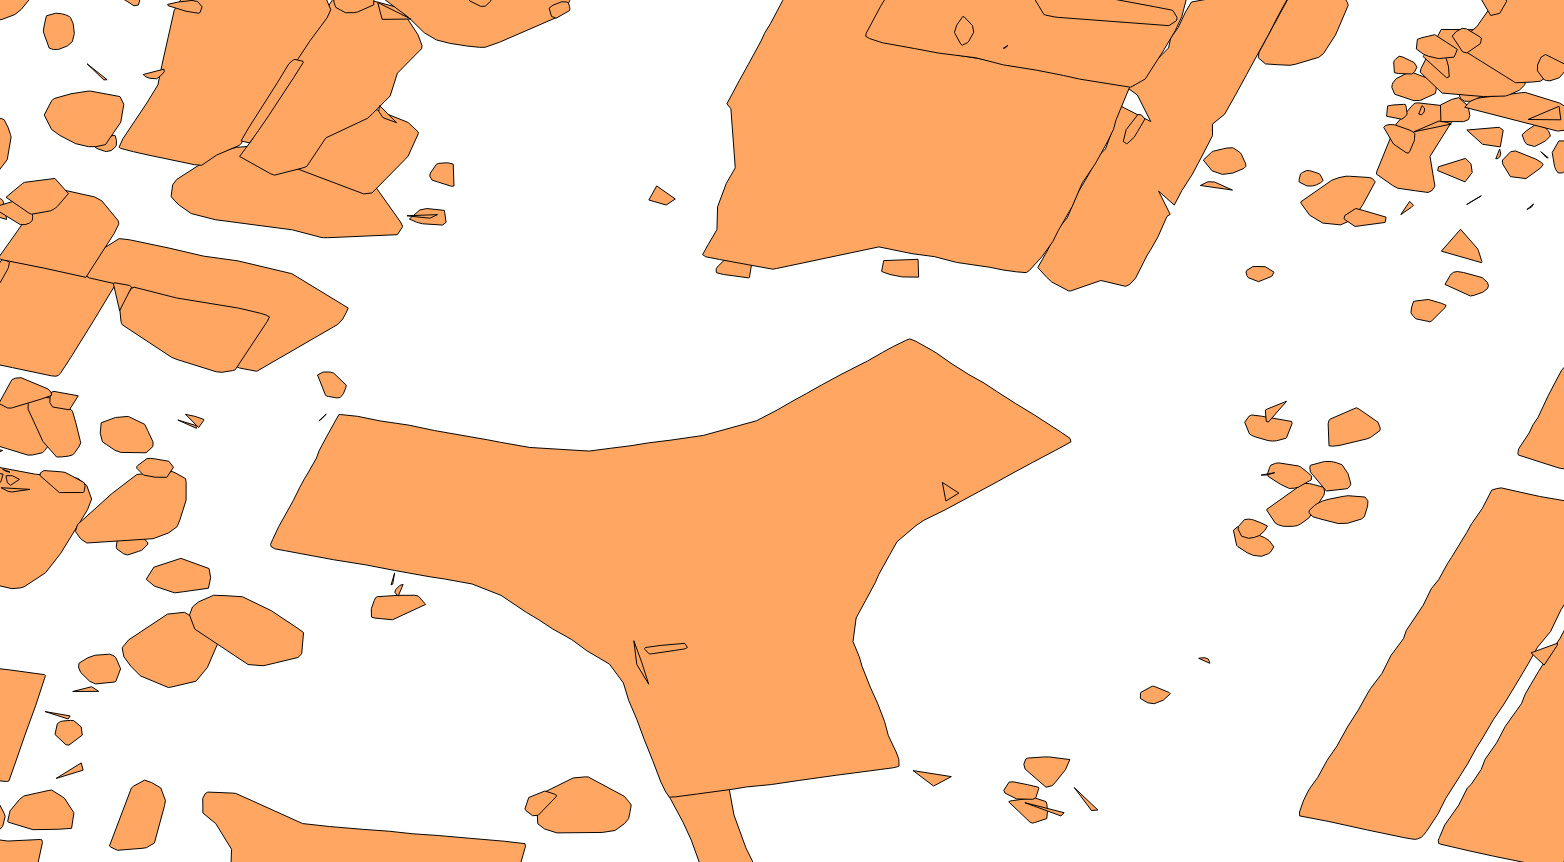
\includegraphics[width=\linewidth]{img/wynik_naiwny_eti.png}
        \caption{Wynik działania algorytmu}
    \end{subfigure}%
    \begin{subfigure}[b]{0.5\linewidth}
        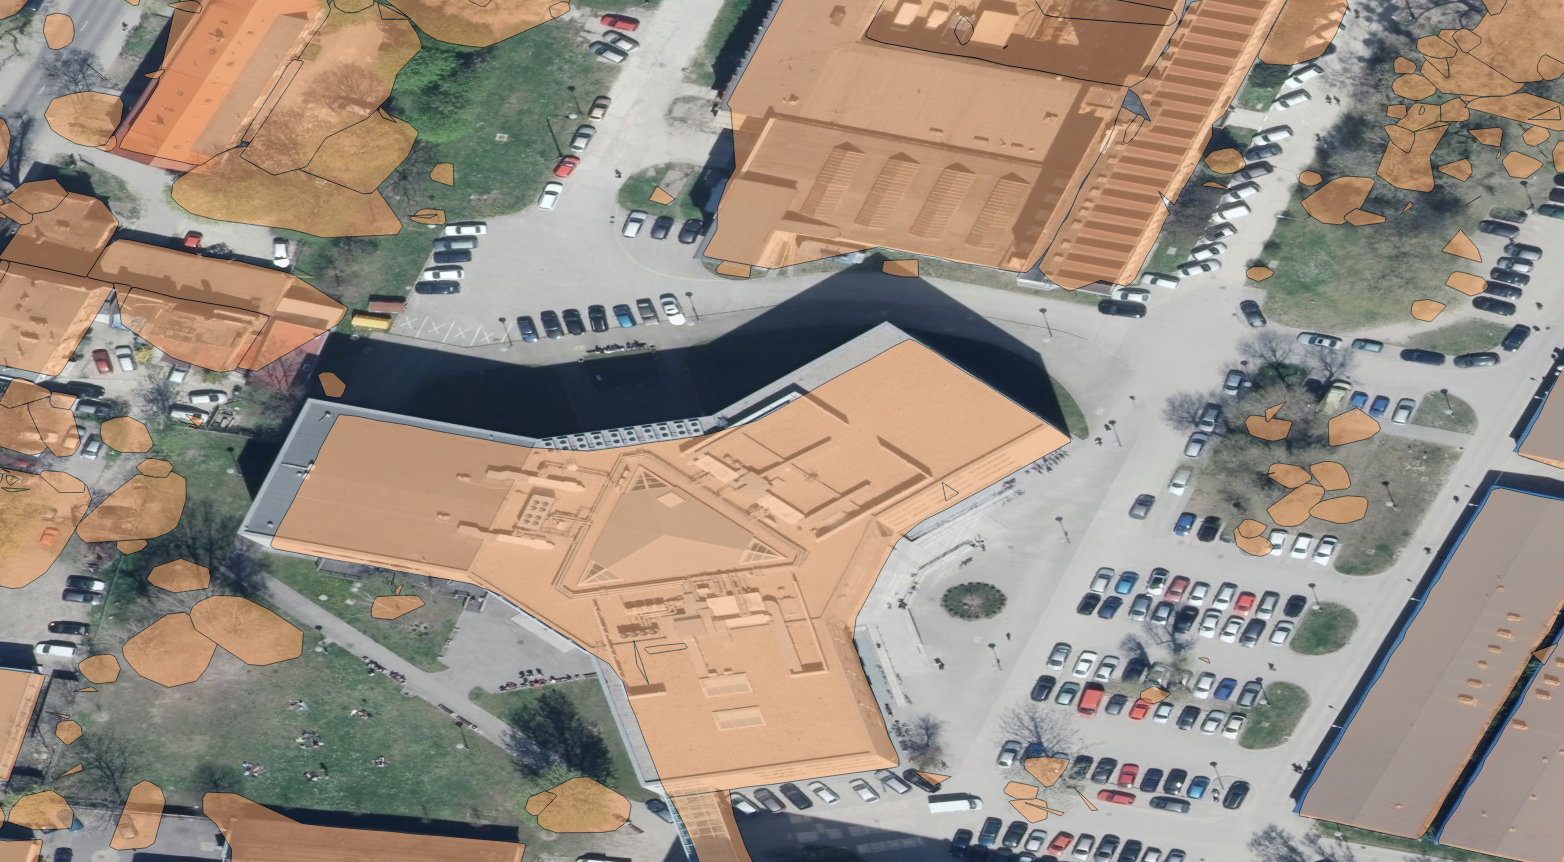
\includegraphics[width=\linewidth]{img/wynik_naiwny_eti_real.png}
        \caption{Wynik po nałożeniu na zdjęcie}
    \end{subfigure}%
    \caption{Zbliżenie na gmach ETI}
    \source{http://mapy.geoportal.gov.pl/wss/service/img/guest/ORTO/MapServer/WMSServer}
    \label{fig:wynik_naiwny_eti}
\end{figure}

Na rysunku \ref{fig:wynik_naiwny_eti} przedstawiono wyniki działania algorytmu naiwnego po
zbliżeniu na obszar wokół nowego gmachu ETI. Widać, że obrysy: budynku OiO (górna część zdjęcia)
oraz baraków (prawa strona zdjęcia) zostały obliczone idealnie. Obrys gmachu nowego ETI także ma
odpowiedni kształt, jednakże wydaje się być nieco przesunięty względem faktycznego położenia budynku.


\begin{figure}[h!]
    \centering
    \begin{subfigure}[b]{0.5\linewidth}
        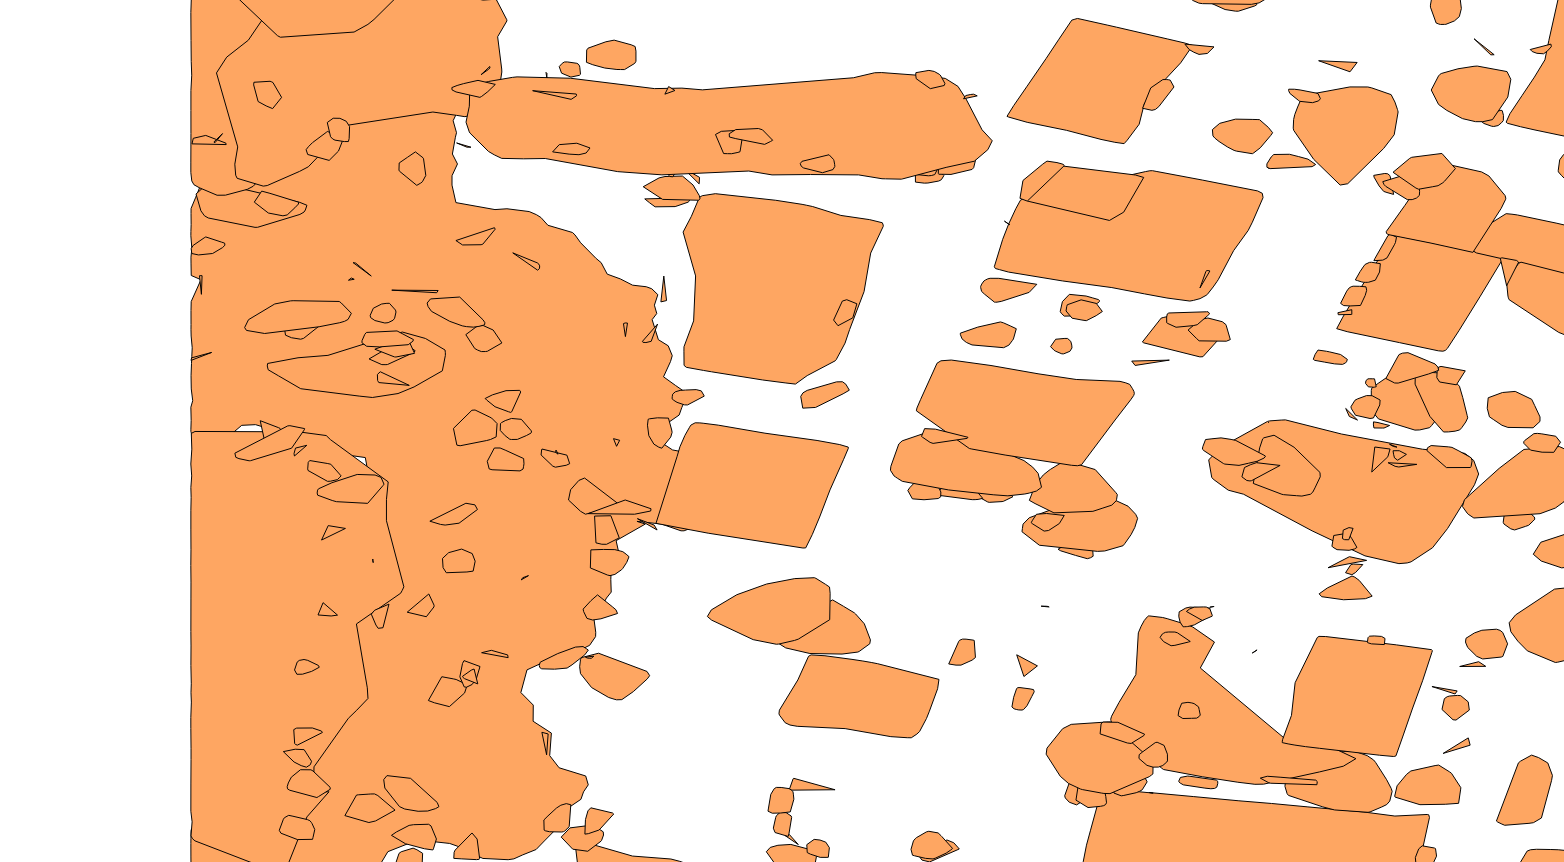
\includegraphics[width=\linewidth]{img/wynik_naiwny_las.png}
        \caption{Wynik działania algorytmu}
    \end{subfigure}%
    \begin{subfigure}[b]{0.5\linewidth}
        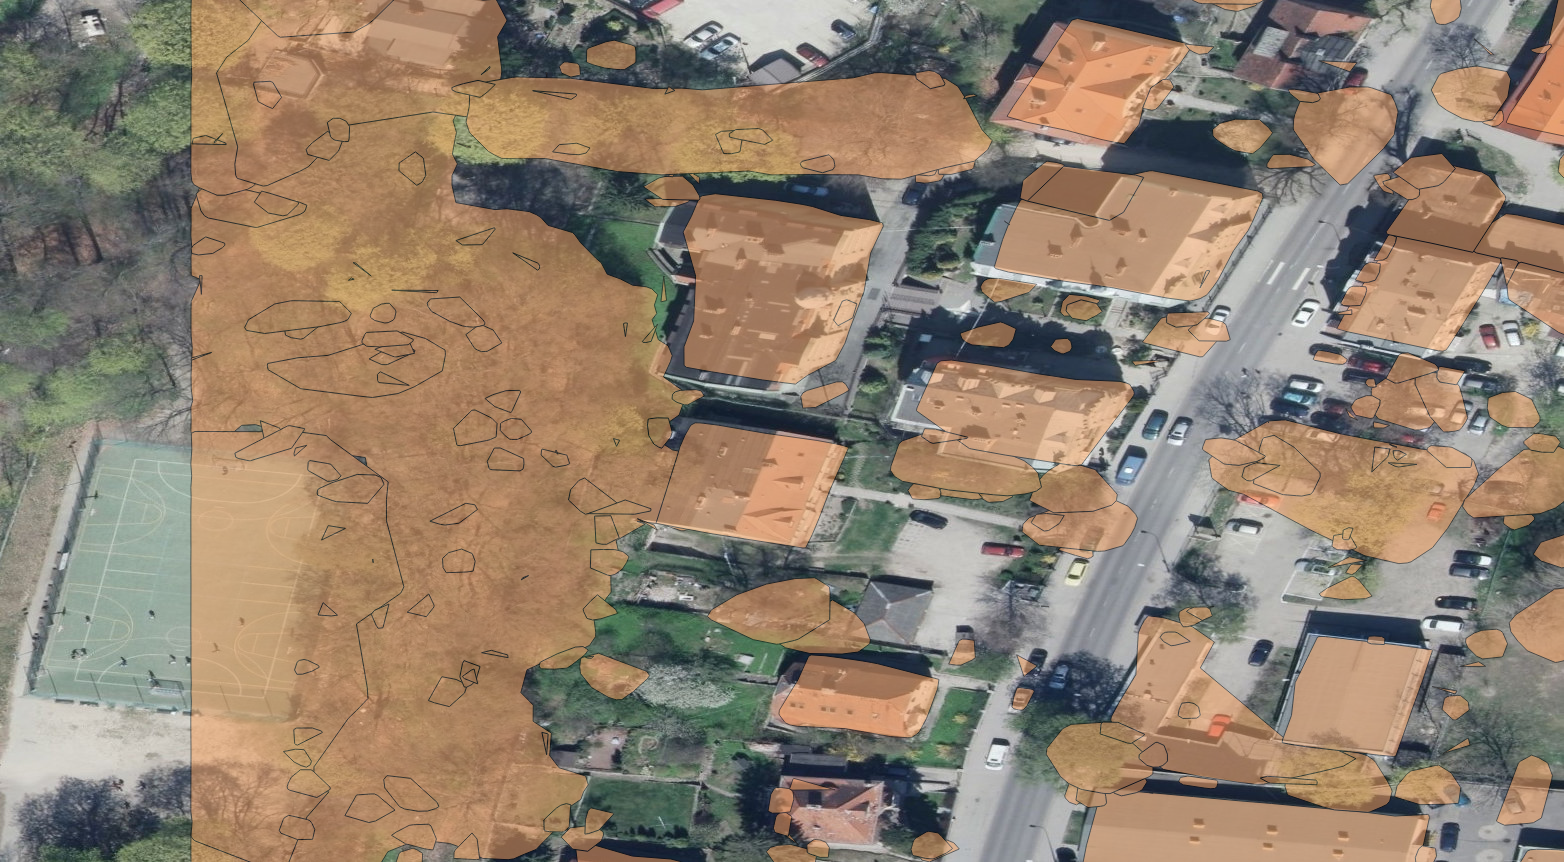
\includegraphics[width=\linewidth]{img/wynik_naiwny_las_real.png}
        \caption{Wynik po nałożeniu na zdjęcie}
    \end{subfigure}%
    \caption{Zbliżenie na tereny zalesione}
    \source{http://mapy.geoportal.gov.pl/wss/service/img/guest/ORTO/MapServer/WMSServer}
    \label{fig:wynik_naiwny_las}
\end{figure}

Na rysunku \ref{fig:wynik_naiwny_las} przedstawiono wynik działania algorytmu naiwnego po
zbliżeniu na obszar zalesiony. Niestety w takim środowisku program radzi sobie znacznie gorzej.
Wykrył bardzo duży obszar leśny jako jedną powierzchnię, w której znajdują się inne, mniejsze.
Jednocześnie widoczne na zdjęciu boisko zostało zakwalifikowane do jednego zbioru razem z 
przyległymi drzewami.

Po analizie z wykorzystaniem algorytmu naiwnego przetestowano algorytm iteracyjny.

\begin{figure}[h!]
    \centering
    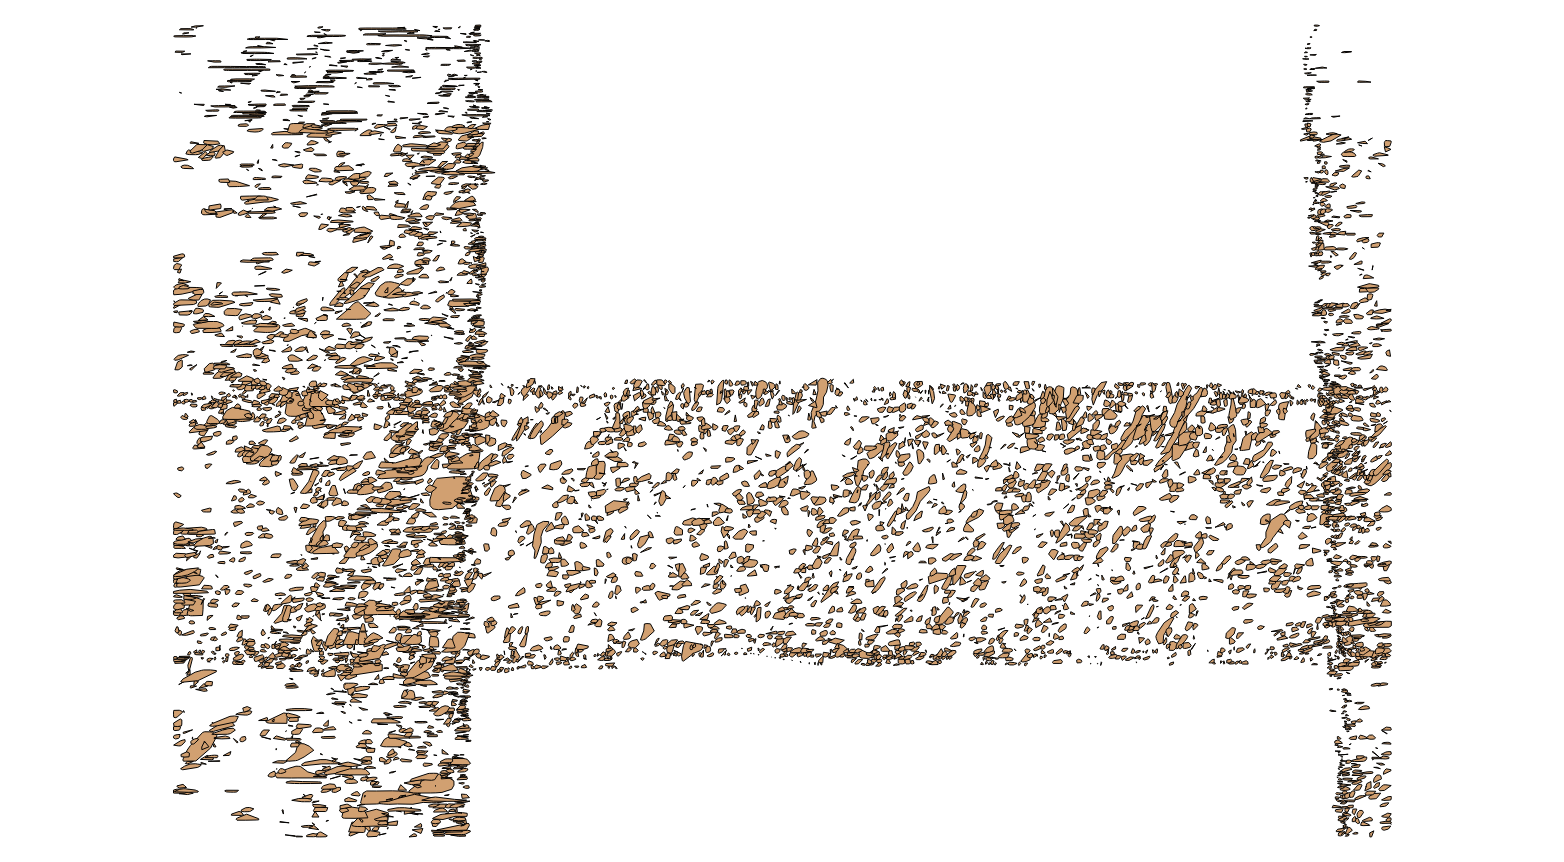
\includegraphics[width=0.5\linewidth]{img/wynik_iter1.png}
    \caption{Efekt działania algorytmu iteracyjnego (1 iteracja)}
    \label{fig:wynik_iteracyjny}
\end{figure}

Jak widać na rysunku \ref{fig:wynik_iteracyjny} po pierwszej iteracji otrzymane wyniki
znacznie odbiegają od tego, co faktycznie znajduje się na danych testowych. Jednakże
było to spodziewane po eksperymentach przeprowadzonyc na danych generowanych. Dlatego przeprowadzono
wiecej iteracji.

\begin{figure}[h!]
    \centering
    \begin{subfigure}[b]{0.5\linewidth}
        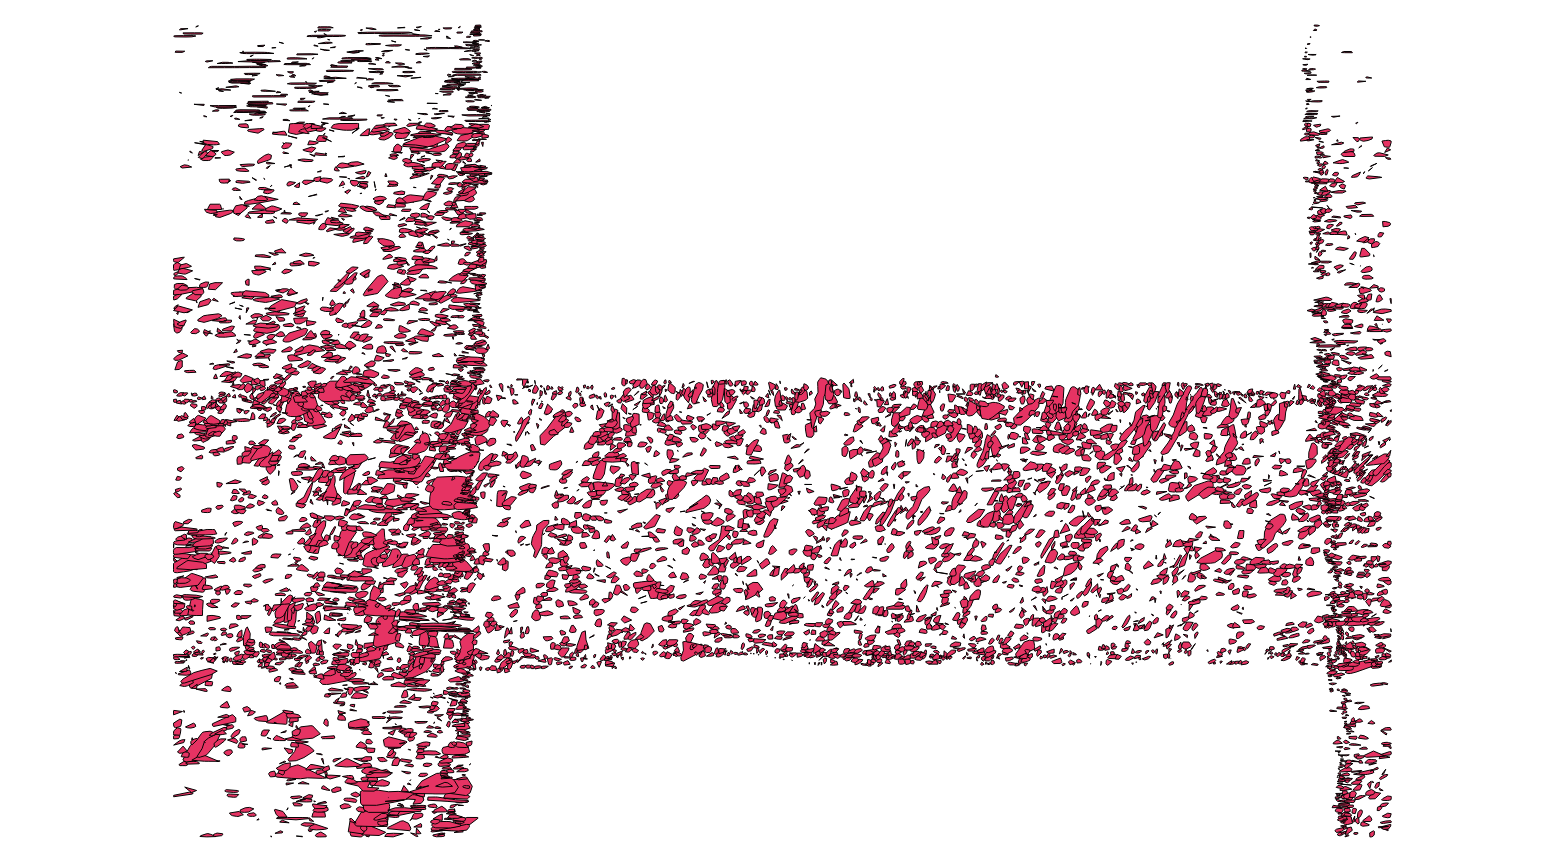
\includegraphics[width=\linewidth]{img/wynik_iter2.png}
        \caption{Efekt działania algorytmu iteracyjnego (2 iteracja)}
    \end{subfigure}%
    \begin{subfigure}[b]{0.5\linewidth}
        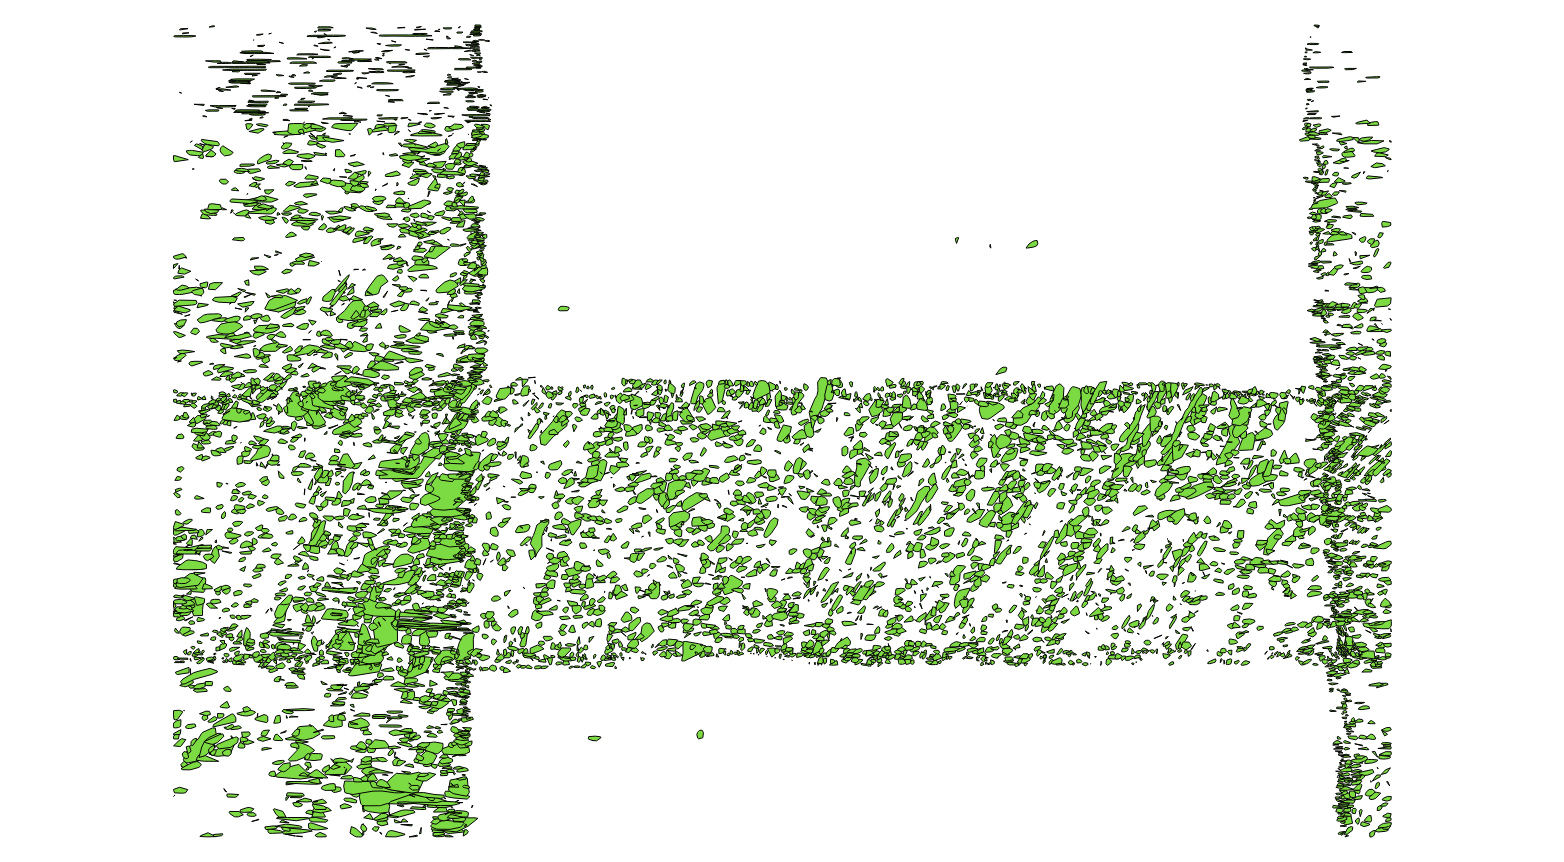
\includegraphics[width=\linewidth]{img/wynik_iter3.png}
        \caption{Efekt działania algorytmu iteracyjnego (3 iteracja)}
    \end{subfigure}%
    \caption{Wyniki kolejnych iteracji}
    \source{http://mapy.geoportal.gov.pl/wss/service/img/guest/ORTO/MapServer/WMSServer}
    \label{fig:wynik_naiwny_las}
\end{figure}

Wraz z kolejnymi iteracjami można zaobserwować pewien postęp (przy trzeciej iteracji
widoczne są nowe obszary), jednakże postęp ten jest niezwykle powolny. Dodając do tego
czasy wykonywania się kolejnych iteracji, przedstawione w tabeli \ref{tab:iter_czasy},
stwierdzono, że algorytm ten nie nadaje się do analizy tak dużych plików.

\begin{table}[h!]
    \centering
    \begin{tabular}{|p{0.5\linewidth}|p{0.5\linewidth}|}
        \hline
		1 iteracja & 15 minut \\
		\hline
		2 iteracje & 35 minut \\
		\hline
		3 iteracje & 1 godzina 15 minut \\
		\hline
    \end{tabular}
    \caption{Czasy wykonywania kolejnych iteracji}
    \label{tab:iter_czasy}
\end{table}


Ostatnim testem było połączenie obu rozwiązań, tzn. najpierw wyszukaniem zbiorów
przy wykorzystaniu algorytmu naiwnego a następnie stopniowym ulepszaniem jego wyniku
poprzez iteracje. Niestety takie podejście okazało się być zbyt czasochłonne 1 iteracja
trwała ponad godzinę, a nie zauważono znacznej poprawy w wynikach. W związku z powyższym
za najlepszy wynik uznano ten uzyskany przez algorytm naiwny.

\section{Omówienie}

Jak pokazały eksperymenty, żadna z metod nie gwarantuje idealnego wykrywania powierzchni. Algorytm
uproszczony ma problemy z prawidłowym wykrywaniem drzew oraz innych struktur charakteryzujących się
nieregularną powierzchnią. Jego wykorzystywanie będzie oznaczać kompresję stratną danych wejściowych.

Algorytm iteracyjny nie dał żadnych prawidłowych wyników. Co prawda dla danych sztucznie wygenerowanych
był w stanie prawidłow sklasyfikować dane do dwóch różnych powierzchni, lecz przy próbie wykorzystania
danych prawdziwych po kliku iteracjach wynik jest daleki od tego, co oferuje algorytm naiwny. Mozna
domniemywać, że za ten stan rzeczy odpowiedzialna jest niedostateczna ilość iteracji. Niestety, wraz
z każdą iteracją rośnie też średni czas jej obliczania. Sprawia to, że algorytm ten w zaproponowanej formie
jest bezużyteczny do analizy danych LiDAR.

Ostatecznie zdecydowane, że to algorytm naiwny daje akceptowalne wyniki. Rezultat działania tego algorytmu,
po przekonwertowaniu do formatu SHP waży poniżej 1MB, co oznacza zmniejszenie wagi danych niemalże 180 razy.
Pliki takiej wielkości można szybko przesyłać poprzez sieć. Pokazuje to, że algorytm naiwny może znaleźć
zatosowanie przy tworzenie systemu web-GIS do udostępniania danych LiDAR.
